% Отчёт по лабораторной работе: Построение простой линейной регрессии
\documentclass[12pt,a4paper]{article}
\usepackage[utf8]{inputenc}
\usepackage[T2A]{fontenc}
\usepackage[russian]{babel}
\usepackage{amsmath,amssymb}
\usepackage{graphicx}
\usepackage{longtable}
\usepackage{booktabs}
\usepackage{geometry}
\usepackage{caption}
\geometry{left=25mm,right=25mm,top=25mm,bottom=25mm}

\title{Лабораторная работа: Построение простой линейной регрессии}
\author{Вариант 1}
\date{\today}

\begin{document}
\maketitle

\section*{Цель работы}
Построить простую линейную регрессию для заданной выборки, оценить коэффициенты регрессии, построить доверительные интервалы и сделать статистические выводы.

\section{Данные}
Файл с данными: \texttt{variant\_1\_data.csv}. Ниже приведена таблица исходных наблюдений (i, x, y).

\begin{longtable}{rrr}
\toprule
 i & x & y \\
\midrule
\endfirsthead
\toprule
 i & x & y \\
\midrule
\endhead
\bottomrule
\endfoot
 1 & 0.7775 & 0.7706 \\
 2 & 1.3653 & 2.0631 \\
 3 & 2.0717 & 4.5496 \\
 4 & 2.3275 & 3.4272 \\
 5 & 2.3641 & 2.9128 \\
 6 & 2.9501 & 4.7224 \\
 7 & 3.2074 & 4.2667 \\
 8 & 3.5111 & 5.5796 \\
 9 & 4.0744 & 4.6881 \\
 10 & 4.2488 & 5.1874 \\
 11 & 4.7173 & 3.0364 \\
 12 & 4.8468 & 4.5618 \\
 13 & 5.4100 & 6.0698 \\
 14 & 5.5097 & 5.3279 \\
 15 & 6.3898 & 6.8934 \\
 16 & 6.8485 & 6.5860 \\
 17 & 7.0493 & 6.5276 \\
 18 & 7.5180 & 7.0654 \\
 19 & 7.7663 & 7.8603 \\
 20 & 8.0611 & 7.2422 \\
 21 & 8.1863 & 7.2499 \\
 22 & 9.0410 & 7.5808 \\
 23 & 9.4203 & 8.0560 \\
 24 & 9.4376 & 8.2323 \\
 25 & 10.1248 & 7.6338 \\
 26 & 10.4685 & 8.4081 \\
 27 & 10.9821 & 8.5309 \\
 28 & 11.3358 & 8.6068 \\
 29 & 11.5871 & 8.6055 \\
 30 & 12.2170 & 10.3130 \\
\end{longtable}

\section{Расчёты характеристик}

\subsection{Средние и суммы квадратов отклонений}

Сначала вычислим средние значения по формулам:
\[
\bar{x} = \frac{1}{n} \sum_{i=1}^{n} x_i = \frac{1}{30} \sum_{i=1}^{30} x_i = 6.460507
\]
\[
\bar{y} = \frac{1}{n} \sum_{i=1}^{n} y_i = \frac{1}{30} \sum_{i=1}^{30} y_i = 6.085180
\]

Далее рассчитаем суммы квадратов отклонений:
\[
S_{xx} = \sum_{i=1}^{n} (x_i - \bar{x})^2 = 327.493632
\]
\[
S_{xy} = \sum_{i=1}^{n} (x_i - \bar{x})(y_i - \bar{y}) = 206.729514
\]

\subsection{Оценки коэффициентов регрессии}

По методу наименьших квадратов:
\[
\hat{\beta}_1 = \frac{S_{xy}}{S_{xx}} = \frac{206.729514}{327.493632} = 0.631247
\]
\[
\hat{\beta}_0 = \bar{y} - \hat{\beta}_1 \bar{x} = 6.085180 - 0.631247 \times 6.460507 = 2.007002
\]

Уравнение регрессии: $\hat{y} = 2.0070 + 0.6312\,x$

Интерпретация: при увеличении $x$ на 1 единицу значение $y$ в среднем увеличивается на 0.6312 единиц.

\subsection{Остатки и остаточная сумма квадратов}

Остатки (residuals) рассчитываются как отклонения фактических значений от прогнозируемых:
\[
e_i = y_i - \hat{y}_i
\]

Таблица прогнозных значений и остатков:

\begin{longtable}{rrrrr}
\toprule
$i$ & $x_i$ & $y_i$ & $\hat{y}_i$ & $e_i$ & $e_i^2$ \\
\midrule
\endfirsthead
\toprule
$i$ & $x_i$ & $y_i$ & $\hat{y}_i$ & $e_i$ & $e_i^2$ \\
\midrule
\endhead
\bottomrule
\endfoot
  1 & 0.7775 &  0.7706 &  2.4978 & -1.7272 & 2.9831 \\
  2 & 1.3653 &  2.0631 &  2.8688 & -0.8057 & 0.6492 \\
  3 & 2.0717 &  4.5496 &  3.3148 &  1.2348 & 1.5248 \\
  4 & 2.3275 &  3.4272 &  3.4762 & -0.0490 & 0.0024 \\
  5 & 2.3641 &  2.9128 &  3.4993 & -0.5865 & 0.3440 \\
  6 & 2.9501 &  4.7224 &  3.8692 &  0.8532 & 0.7279 \\
  7 & 3.2074 &  4.2667 &  4.0317 &  0.2350 & 0.0552 \\
  8 & 3.5111 &  5.5796 &  4.2234 &  1.3562 & 1.8393 \\
  9 & 4.0744 &  4.6881 &  4.5790 &  0.1091 & 0.0119 \\
 10 & 4.2488 &  5.1874 &  4.6890 &  0.4984 & 0.2484 \\
 11 & 4.7173 &  3.0364 &  4.9848 & -1.9484 & 3.7962 \\
 12 & 4.8468 &  4.5618 &  5.0665 & -0.5047 & 0.2548 \\
 13 & 5.4100 &  6.0698 &  5.4221 &  0.6477 & 0.4196 \\
 14 & 5.5097 &  5.3279 &  5.4850 & -0.1571 & 0.0247 \\
 15 & 6.3898 &  6.8934 &  6.0405 &  0.8529 & 0.7274 \\
 16 & 6.8485 &  6.5860 &  6.3301 &  0.2559 & 0.0655 \\
 17 & 7.0493 &  6.5276 &  6.4569 &  0.0707 & 0.0050 \\
 18 & 7.5180 &  7.0654 &  6.7527 &  0.3127 & 0.0978 \\
 19 & 7.7663 &  7.8603 &  6.9095 &  0.9508 & 0.9041 \\
 20 & 8.0611 &  7.2422 &  7.0956 &  0.1466 & 0.0215 \\
 21 & 8.1863 &  7.2499 &  7.1746 &  0.0753 & 0.0057 \\
 22 & 9.0410 &  7.5808 &  7.7141 & -0.1333 & 0.0178 \\
 23 & 9.4203 &  8.0560 &  7.9535 &  0.1025 & 0.0105 \\
 24 & 9.4376 &  8.2323 &  7.9645 &  0.2678 & 0.0717 \\
 25 & 10.1248 &  7.6338 &  8.3983 & -0.7645 & 0.5844 \\
 26 & 10.4685 &  8.4081 &  8.6152 & -0.2071 & 0.0429 \\
 27 & 10.9821 &  8.5309 &  8.9394 & -0.4085 & 0.1669 \\
 28 & 11.3358 &  8.6068 &  9.1627 & -0.5559 & 0.3090 \\
 29 & 11.5871 &  8.6055 &  9.3213 & -0.7158 & 0.5124 \\
 30 & 12.2170 & 10.3130 &  9.7190 &  0.5940 & 0.3529 \\
\end{longtable}

Остаточная сумма квадратов (RSS):
\[
\text{RSS} = \sum_{i=1}^{n} e_i^2 = 16.777049
\]

\subsection{Оценка дисперсии ошибок и стандартные ошибки}

Оценка дисперсии ошибок:
\[
s^2 = \frac{\text{RSS}}{n-2} = \frac{16.777049}{30-2} = \frac{16.777049}{28} = 0.599180
\]

Остаточное стандартное отклонение:
\[
s = \sqrt{s^2} = \sqrt{0.599180} = 0.774067
\]

Стандартная ошибка для $\hat{\beta}_1$:
\[
\text{SE}(\hat{\beta}_1) = \frac{s}{\sqrt{S_{xx}}} = \frac{0.774067}{\sqrt{327.493632}} = \frac{0.774067}{18.0971} = 0.042774
\]

Стандартная ошибка для $\hat{\beta}_0$:
\[
\text{SE}(\hat{\beta}_0) = s \sqrt{\frac{1}{n} + \frac{\bar{x}^2}{S_{xx}}} = 0.774067 \sqrt{\frac{1}{30} + \frac{(6.460507)^2}{327.493632}} = 0.310381
\]

\subsection{Доверительные интервалы для коэффициентов}

На уровне значимости $\alpha = 0.05$ критическое значение распределения Стьюдента с числом степеней свободы $df = n-2 = 28$:
\[
t_{1-\alpha/2, \, df=28} = t_{0.975, 28} = 2.0484
\]

95\% доверительный интервал для $\beta_0$:
\[
\hat{\beta}_0 \pm t \cdot \text{SE}(\hat{\beta}_0) = 2.007002 \pm 2.0484 \times 0.310381 = [1.3712, \, 2.6428]
\]

95\% доверительный интервал для $\beta_1$:
\[
\hat{\beta}_1 \pm t \cdot \text{SE}(\hat{\beta}_1) = 0.631247 \pm 2.0484 \times 0.042774 = [0.5436, \, 0.7189]
\]

\textbf{Вывод о значимости:} Ноль не попадает в доверительный интервал для $\beta_1$, следовательно, коэффициент наклона $\beta_1$ статистически значимо отличается от нуля при уровне значимости $\alpha = 0.05$. Это подтверждает значимость линейной зависимости.

\subsection{Коэффициент детерминации}

Общая сумма квадратов:
\[
\text{TSS} = \sum_{i=1}^{n} (y_i - \bar{y})^2 = 147.274524
\]

Коэффициент детерминации:
\[
R^2 = 1 - \frac{\text{RSS}}{\text{TSS}} = 1 - \frac{16.777049}{147.274524} = 0.8861 \quad (88.61\%)
\]

Интерпретация: модель объясняет 88.61\% вариации зависимой переменной $y$. Это указывает на хорошее качество модели.

\section{Построение графиков}
Ниже представлены графики: диаграмма рассеяния и оценённая прямая с 95\% доверительным интервалом.

\begin{figure}[ht]
\centering
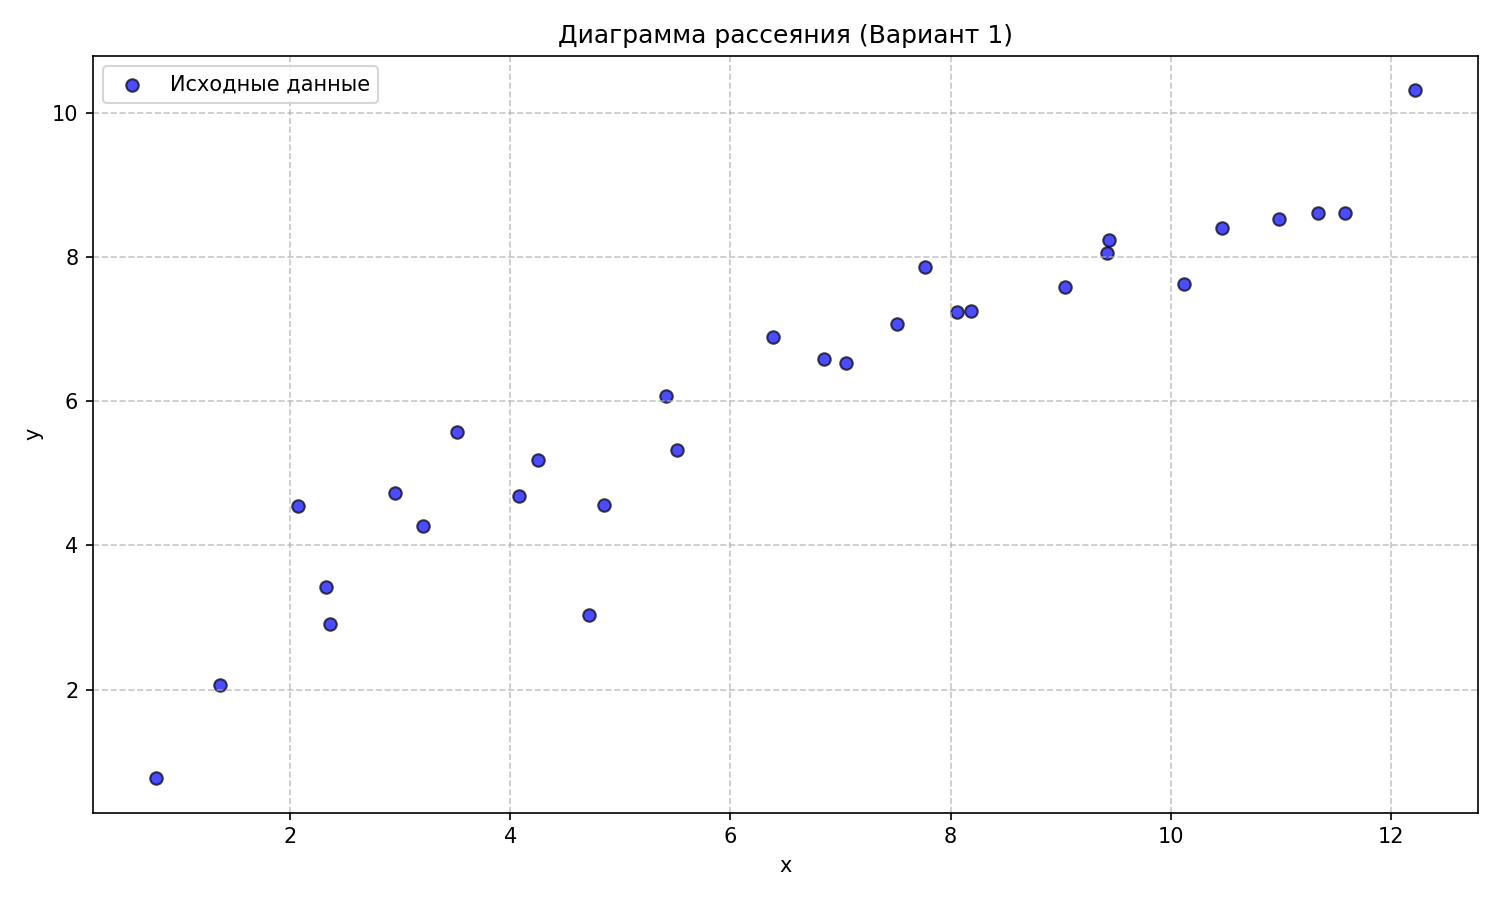
\includegraphics[width=0.7\textwidth]{scatter_plot.png}
\caption{Диаграмма рассеяния (Вариант 1)}
\end{figure}

\begin{figure}[ht]
\centering
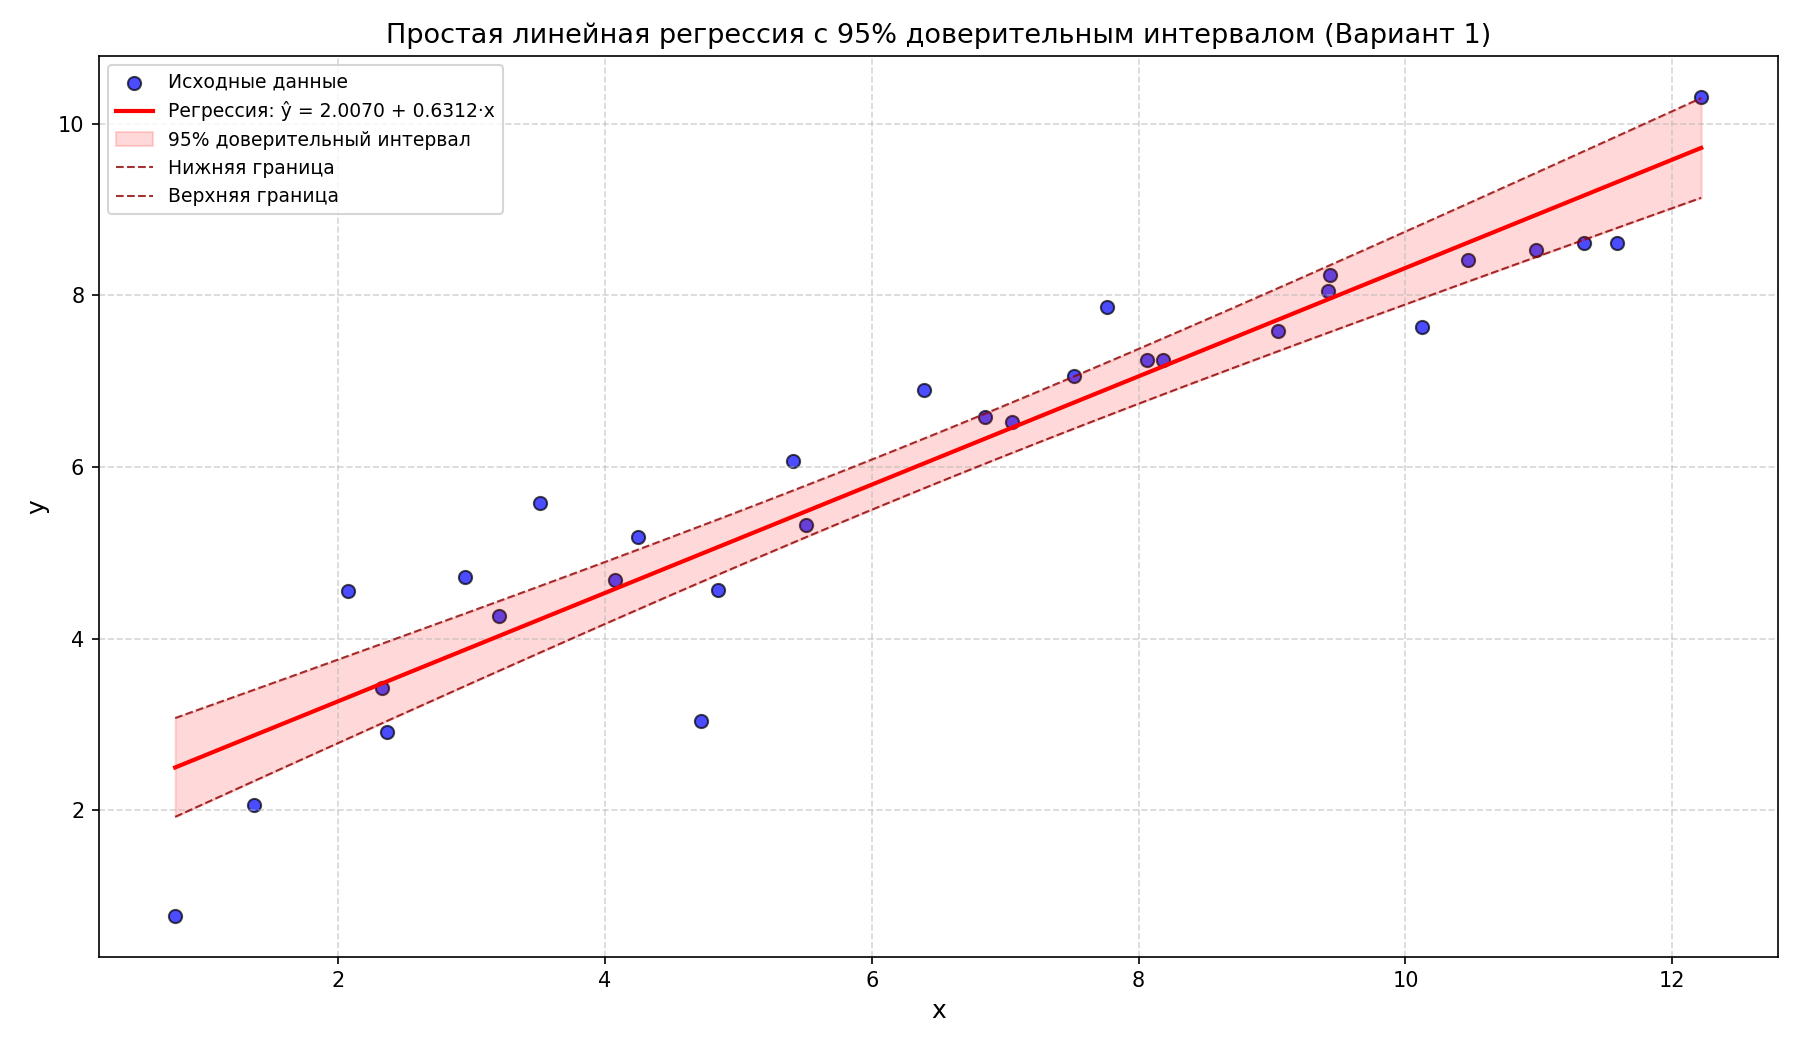
\includegraphics[width=0.8\textwidth]{regression_with_CI.png}
\caption{Простая линейная регрессия с 95\% доверительным интервалом}
\end{figure}

\subsection{Анализ диаграммы рассеяния}

Диаграмма рассеяния (рис. 1) показывает, что между переменными $x$ и $y$ наблюдается явная положительная линейная зависимость. Точки в целом следуют линейному тренду: с увеличением $x$ значения $y$ тенденциально возрастают. Это визуально подтверждает целесообразность применения простой линейной регрессии.

\subsection{Анализ графика регрессии и доверительного интервала}

На графике регрессии с 95\% доверительным интервалом (рис. 2) видны следующие особенности:

\begin{enumerate}
\item \textbf{Узкий интервал вблизи среднего значения.} Доверительный интервал имеет минимальную ширину (наиболее узкий) в той области графика, где $x$ близок к среднему значению $\bar{x} = 6.4605$. Это объясняется формулой стандартной ошибки:
\[
\text{SE}(\hat{y}(x_0)) = s \sqrt{\frac{1}{n} + \frac{(x_0 - \bar{x})^2}{S_{xx}}}
\]
При $x_0 = \bar{x}$ второе слагаемое под корнем обнуляется, стандартная ошибка минимальна.

\item \textbf{Расширение интервала при удалении от центра.} По мере удаления $x_0$ от $\bar{x}$ (как влево, так и вправо) терм $(x_0 - \bar{x})^2$ возрастает, и доверительный интервал расширяется. Это создаёт характерную форму, напоминающую «песочные часы» или расширяющуюся воронку.

\item \textbf{Уверенность в прогнозе в центре диапазона.} Прогноз является наиболее точным при значениях $x$, близких к $\bar{x}$, где накоплено больше информации (в смысле дисперсии).

\item \textbf{Неуверенность при экстраполяции.} На концах диапазона (особенно за пределами наблюдаемых значений) интервал существенно расширяется, что предостерегает от экстраполяции.
\end{enumerate}

\subsection{Характеристика качества модели по графику}

\begin{enumerate}
\item \textbf{Наблюдаемые точки и линия регрессии:} На графике видно, что точки данных достаточно тесно группируются вокруг оценённой линии регрессии. Большинство точек находятся вблизи прямой, что говорит о хорошей аппроксимации моделью.

\item \textbf{Остатки и случайность:} Визуальный осмотр показывает, что остатки (вертикальные отклонения точек от линии) распределяются относительно случайно, без видимого систематического тренда. Это подтверждает предположение о независимости и одинаковости распределения ошибок (гомоскедастичность).

\item \textbf{Коэффициент детерминации:} $R^2 = 0.8861 = 88.61\%$ означает, что модель объясняет почти 89\% доли дисперсии отклика. По шкале:
\begin{itemize}
\item $R^2 < 0.5$ — низкое качество;
\item $0.5 \le R^2 < 0.7$ — среднее качество;
\item $0.7 \le R^2 < 0.9$ — хорошее качество;
\item $R^2 \ge 0.9$ — отличное качество.
\end{itemize}
В нашем случае $R^2 = 0.8861$ соответствует диапазону хорошего качества.

\item \textbf{Диапазон прогнозируемых значений:} Оценённая регрессионная прямая охватывает диапазон от $\approx 2.5$ (при $x \approx 0.8$) до $\approx 9.7$ (при $x \approx 12.2$), что разумно соответствует наблюдаемому диапазону $y \in [0.77, 10.31]$.

\item \textbf{Вывод:} Построенная линейная модель адекватна для данной выборки и может использоваться для прогнозирования значений $y$ при заданных $x$ в диапазоне наблюдаемых данных.
\end{enumerate}

\section{Итоговая сводка результатов}

\begin{table}[ht]
\centering
\begin{tabular}{|l|r|}
\hline
\textbf{Показатель} & \textbf{Значение} \\
\hline
Объём выборки $n$ & 30 \\
Среднее $x$ & 6.460507 \\
Среднее $y$ & 6.085180 \\
$S_{xx}$ & 327.493632 \\
$S_{xy}$ & 206.729514 \\
\hline
$\hat{\beta}_0$ & 2.007002 \\
$\hat{\beta}_1$ & 0.631247 \\
\hline
RSS & 16.777049 \\
TSS & 147.274524 \\
$s^2$ & 0.599180 \\
$s$ & 0.774067 \\
\hline
$\text{SE}(\hat{\beta}_0)$ & 0.310381 \\
$\text{SE}(\hat{\beta}_1)$ & 0.042774 \\
$t_{0.975, 28}$ & 2.0484 \\
\hline
95\% ДИ для $\beta_0$ & [1.3712, 2.6428] \\
95\% ДИ для $\beta_1$ & [0.5436, 0.7189] \\
\hline
$R^2$ & 0.8861 (88.61\%) \\
\hline
\end{tabular}
\caption{Сводка основных результатов анализа}
\end{table}

\section{Статистические выводы}
\begin{enumerate}
\item Коэффициент наклона $\hat{\beta}_1 = 0.6312 > 0$, следовательно зависимость между $x$ и $y$ положительная.
\item Ноль не попадает в 95\% доверительный интервал для $\beta_1$, поэтому линейная зависимость статистически значима на уровне $\alpha=0.05$.
\item Модель объясняет примерно 88.6\% изменчивости зависимой переменной $y$ — качество модели можно считать хорошим.
\end{enumerate}

\section*{Заключение}
Построена простая линейная модель, проведены необходимые оценки и сделаны статистически обоснованные выводы. Графическое представление подтверждает адекватность выбранной модели для текущей выборки.

\vspace{10mm}
\noindent Приложения: исходный код \texttt{main (2).py}, файл с данными \texttt{variant_1_data.csv}, сгенерированные графики \texttt{scatter_plot.png} и \texttt{regression_with_CI.png}.

\end{document}

